\documentclass[12pt,t]{beamer}
\usepackage{geometry}\geometry{paperwidth=10cm,paperheight=17.78cm}
\usepackage{tcolorbox}\tcbuselibrary{skins}
\usepackage{amsmath,amssymb}
\usepackage{tikz}\usetikzlibrary{arrows.meta,calc}
\usepackage{graphicx,xcolor}
\usepackage{xeCJK}\setCJKmainfont{Noto Sans CJK SC}\setCJKsansfont{Noto Sans CJK SC}\setCJKmonofont{Noto Sans CJK SC}
\definecolor{INK}{HTML}{1D1D1F}\definecolor{INK2}{HTML}{6B7280}
\definecolor{ACCENT}{HTML}{E63946}\definecolor{NAVY}{HTML}{1D3557}
\definecolor{SOFTBG}{HTML}{F1F3F5}\definecolor{GOLD}{HTML}{FFF8E1}\definecolor{IBC}{HTML}{2A9D8F}
\definecolor{WM}{HTML}{9AA3AD}
\setbeamertemplate{navigation symbols}{}
\setbeamersize{text margin left=0.5cm,text margin right=0.5cm}
\setbeamercolor{normal text}{fg=INK}
% 每页页脚品牌水印（覆盖 [plain] 与深色帧）
\setbeamertemplate{background}{%
  \begin{tikzpicture}[overlay,remember picture]
    \node[anchor=south,text=WM,font=\footnotesize\bfseries]
      at ([yshift=3mm]current page.south){\xeCJKsetup{CJKecglue={}}Ryan雷老师｜奥克兰物理数学科学};
  \end{tikzpicture}}
\newcommand{\titlebar}[2][NAVY]{\begin{tcolorbox}[enhanced,colback=#1,colframe=#1,arc=1.5mm,boxrule=0pt,left=4mm,right=4mm,top=2.5mm,bottom=2.5mm,width=\linewidth]\color{white}\large\bfseries #2\end{tcolorbox}\par}
\newcommand{\stepchip}[1]{\colorbox{ACCENT}{\color{white}\large\bfseries #1}\par}
\newcommand{\srcnote}[1]{{\footnotesize\color{INK2}#1}\par}
\newtcolorbox{softcard}{enhanced,colback=SOFTBG,colframe=SOFTBG,arc=1.5mm,boxrule=0pt,width=\linewidth,halign=center,fontupper=\large}
\newtcolorbox{goldbox}{enhanced,colback=GOLD,colframe=ACCENT,boxrule=1.5pt,arc=1.5mm,width=\linewidth,halign=center}
\newtcolorbox{hookbar}{enhanced,colback=ACCENT,colframe=ACCENT,arc=2mm,boxrule=0pt,width=\linewidth,halign=center}
\newtcolorbox{lcard}[1][SOFTBG]{enhanced,colback=#1,colframe=#1,arc=1.5mm,boxrule=0pt,width=\linewidth,top=2.5mm,bottom=2.5mm,left=3mm,right=3mm,fontupper=\normalsize}
\newcommand{\rnum}[1]{\tikz[baseline=(n.base)]\node[circle,fill=ACCENT,text=white,font=\bfseries\small,inner sep=0pt,minimum size=1.35em](n){#1};}
\newcommand{\wnum}[1]{\tikz[baseline=(n.base)]\node[circle,fill=white,text=NAVY,font=\bfseries\small,inner sep=0pt,minimum size=1.35em](n){#1};}
\newcommand{\nnum}[1]{\tikz[baseline=(n.base)]\node[circle,fill=NAVY,text=white,font=\bfseries\small,inner sep=0pt,minimum size=1.35em](n){#1};}
% 截图：手机外框 + 相对坐标 scope
\newcommand{\shotframe}{\draw[INK2!45,line width=0.8pt,rounded corners=5pt](img.south west) rectangle (img.north east);}
% 红框 + 左侧编号：\rbox{x0}{y0}{x1}{y1}{号}
\newcommand{\rbox}[5]{\draw[ACCENT,line width=2pt,rounded corners=2pt](#1,#2) rectangle (#3,#4);
  \node[circle,fill=ACCENT,text=white,font=\bfseries\small,inner sep=0pt,minimum size=1.35em,anchor=east] at ($(#1,#2)!0.5!(#1,#4)+(-0.015,0)$){#5};}

\begin{document}

% ---------- P1 封面 ----------
\begin{frame}[plain]\centering
\begin{hookbar}{\Large\bfseries\color{white}新西兰高中补习 · 家长必看}\end{hookbar}
\medskip
{\fontsize{30}{38}\selectfont\bfseries\textcolor{NAVY}{补习老师的资格}\\\textcolor{ACCENT}{一个名字}\textcolor{NAVY}{就能查}\par}
\medskip
\begin{tikzpicture}
\node[anchor=south west,inner sep=0](img) at (0,0){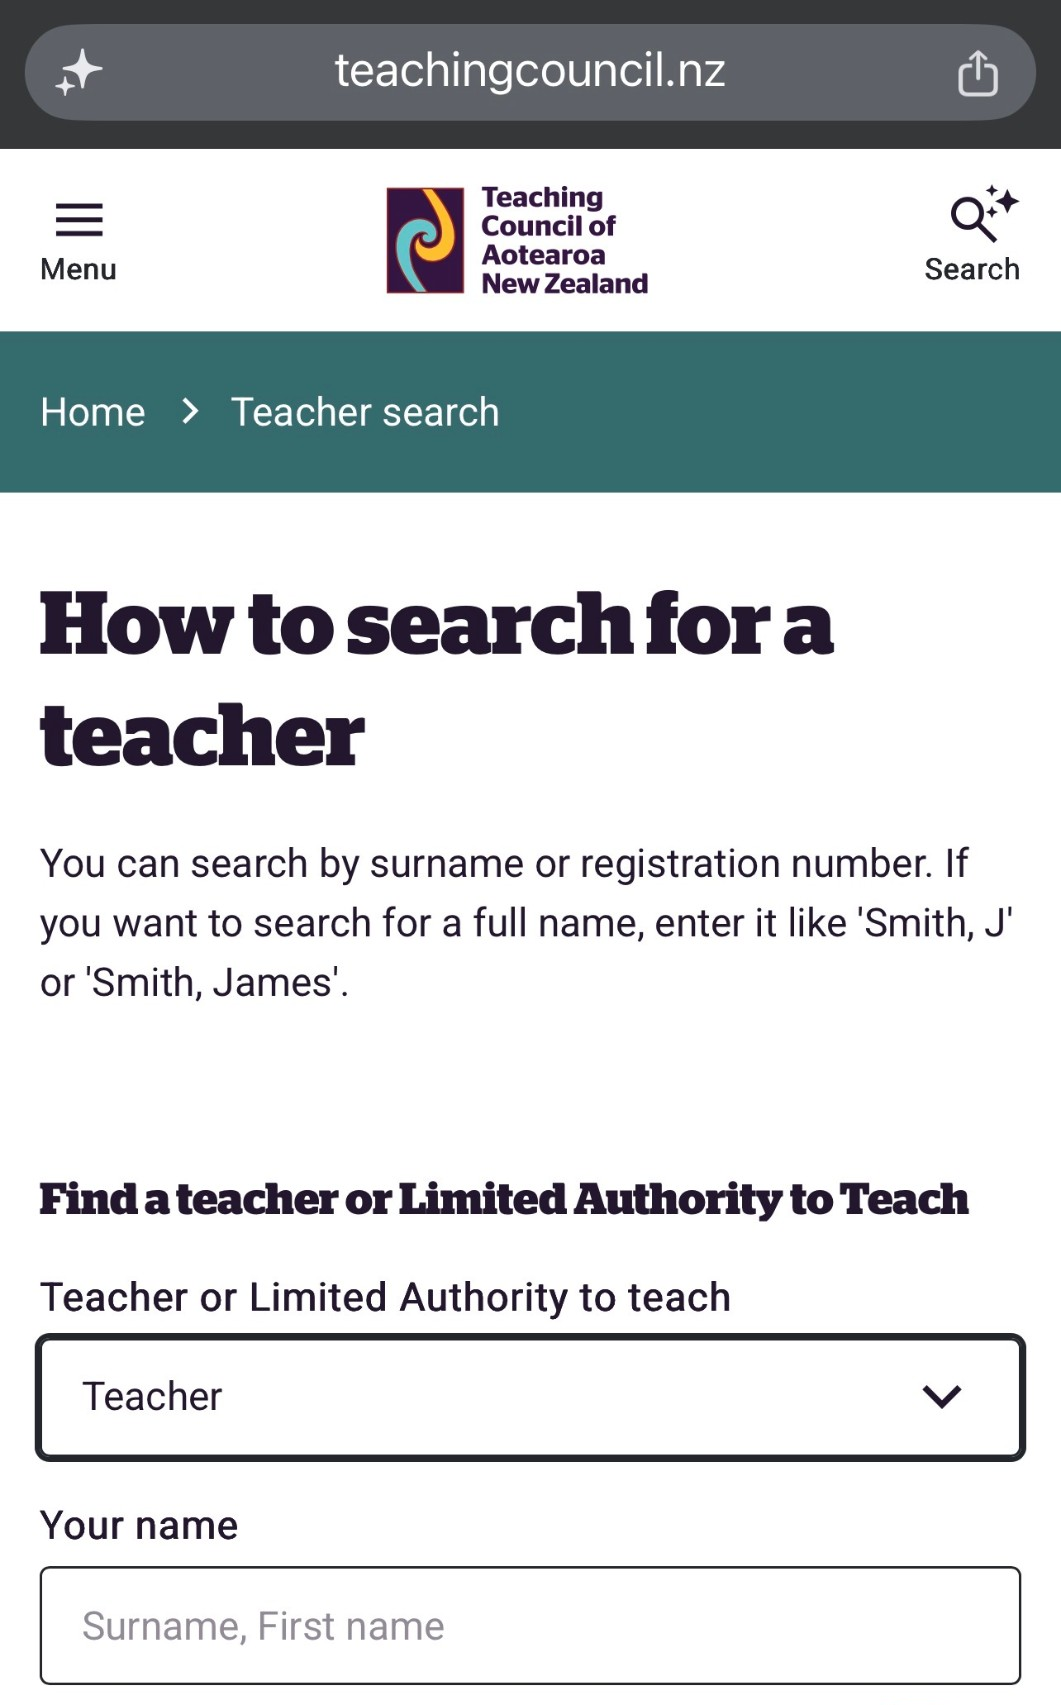
\includegraphics[height=10.6cm]{tutorcheck-tc-02102026}};
\shotframe
\begin{scope}[x={(img.south east)},y={(img.north west)}]
\draw[ACCENT,line width=2.4pt,rounded corners=2pt](0.02,0.004) rectangle (0.98,0.092);
\end{scope}\end{tikzpicture}\par
\smallskip
{\large\color{INK2}两个官网 · 三分钟 · 附操作截图}
\end{frame}

% ---------- P2 一个事实 ----------
\begin{frame}[plain]
\titlebar{先说一件很多家长不知道的事}
\vfill
\begin{goldbox}\centering{\LARGE\bfseries\textcolor{NAVY}{在新西兰做补习}}\\[2mm]{\huge\bfseries\textcolor{ACCENT}{不需要任何执照}}\end{goldbox}
\medskip
\srcnote{新西兰政府职业网站 careers.govt.nz：成为私人补习老师 “no specific requirements”（没有特定要求）}
\vfill
{\large 教师注册，是\textbf{学校}聘老师的门槛；\\[1mm]不是开补习的门槛。\par}
\vfill
{\large 所以简介里的「在职老师」「海外博士」，\\[1mm]可能是真的，也可能只是写写。\par}
\vfill
\begin{lcard}[GOLD]\large 好消息是：有两样，\textbf{官方网站上就能核对}，不用托关系、不用花钱。\end{lcard}
\vfill
{\large\color{INK2}下一页：两个网站，各查一件事 →\par}
\vfill
\end{frame}

% ---------- P3 总览 ----------
\begin{frame}[plain]
\titlebar{两个官网 · 各查一件事}
\vfill
\begin{lcard}
\nnum{1}\hspace{2mm}{\Large\bfseries 是不是新西兰注册教师}\\[2mm]
{\large 网站：\textbf{teachingcouncil.nz}}\\[1mm]
{\large 你需要：\textcolor{ACCENT}{\bfseries 老师的名字}}\\[1mm]
{\color{INK2}全新西兰约 15 万名注册教师，都在这一个库里}
\end{lcard}
\vfill
\begin{lcard}
\nnum{2}\hspace{2mm}{\Large\bfseries 海外学历在新西兰算几级}\\[2mm]
{\large 网站：\textbf{nzqa.govt.nz}（IQA 认证）}\\[1mm]
{\large 你需要：\textcolor{ACCENT}{\bfseries 老师发来的原始 PDF}}\\[1mm]
{\color{INK2}只适用于在海外拿学位的老师}
\end{lcard}
\vfill
\begin{goldbox}\centering{\Large\bfseries\textcolor{NAVY}{第一个只要名字}}\\[1.5mm]{\large 孩子学校的老师，也一样能查}\end{goldbox}
\medskip
\vfill
\srcnote{认准网址：teachingcouncil.nz ｜ nzqa.govt.nz（.govt.nz = 新西兰政府网站）}
\vfill
\end{frame}

% ---------- P4 ① 怎么进 ----------
\begin{frame}[plain]
\titlebar{\wnum{1}\ 教师注册 · 先找到入口}
\medskip\centering
\begin{tikzpicture}
\node[anchor=south west,inner sep=0](img) at (0,0){
\includegraphics[width=0.86\linewidth]{tutorcheck-google-02102026}};
\shotframe
\begin{scope}[x={(img.south east)},y={(img.north west)}]
\rbox{0.03}{0.70}{0.97}{0.79}{1}
\rbox{0.02}{0.33}{0.98}{0.59}{2}
\rbox{0.02}{0.075}{0.98}{0.125}{3}
\end{scope}\end{tikzpicture}\par
\srcnote{截图：Google 搜索结果（已隐去个人头像）}
\medskip\raggedright
{\large\rnum{1}\ Google 搜 \textbf{find a teacher}\par}
\smallskip
{\large\rnum{2}\ 点 Teaching Council 那一条\par}
\smallskip
{\large\rnum{3}\ 约 15 万注册教师，都在这里\par}
\end{frame}

% ---------- P5 ① 输入名字 ----------
\begin{frame}[plain]
\titlebar{\wnum{1}\ 教师注册 · 输入名字}
\medskip\centering
\begin{tikzpicture}
\node[anchor=south west,inner sep=0](img) at (0,0){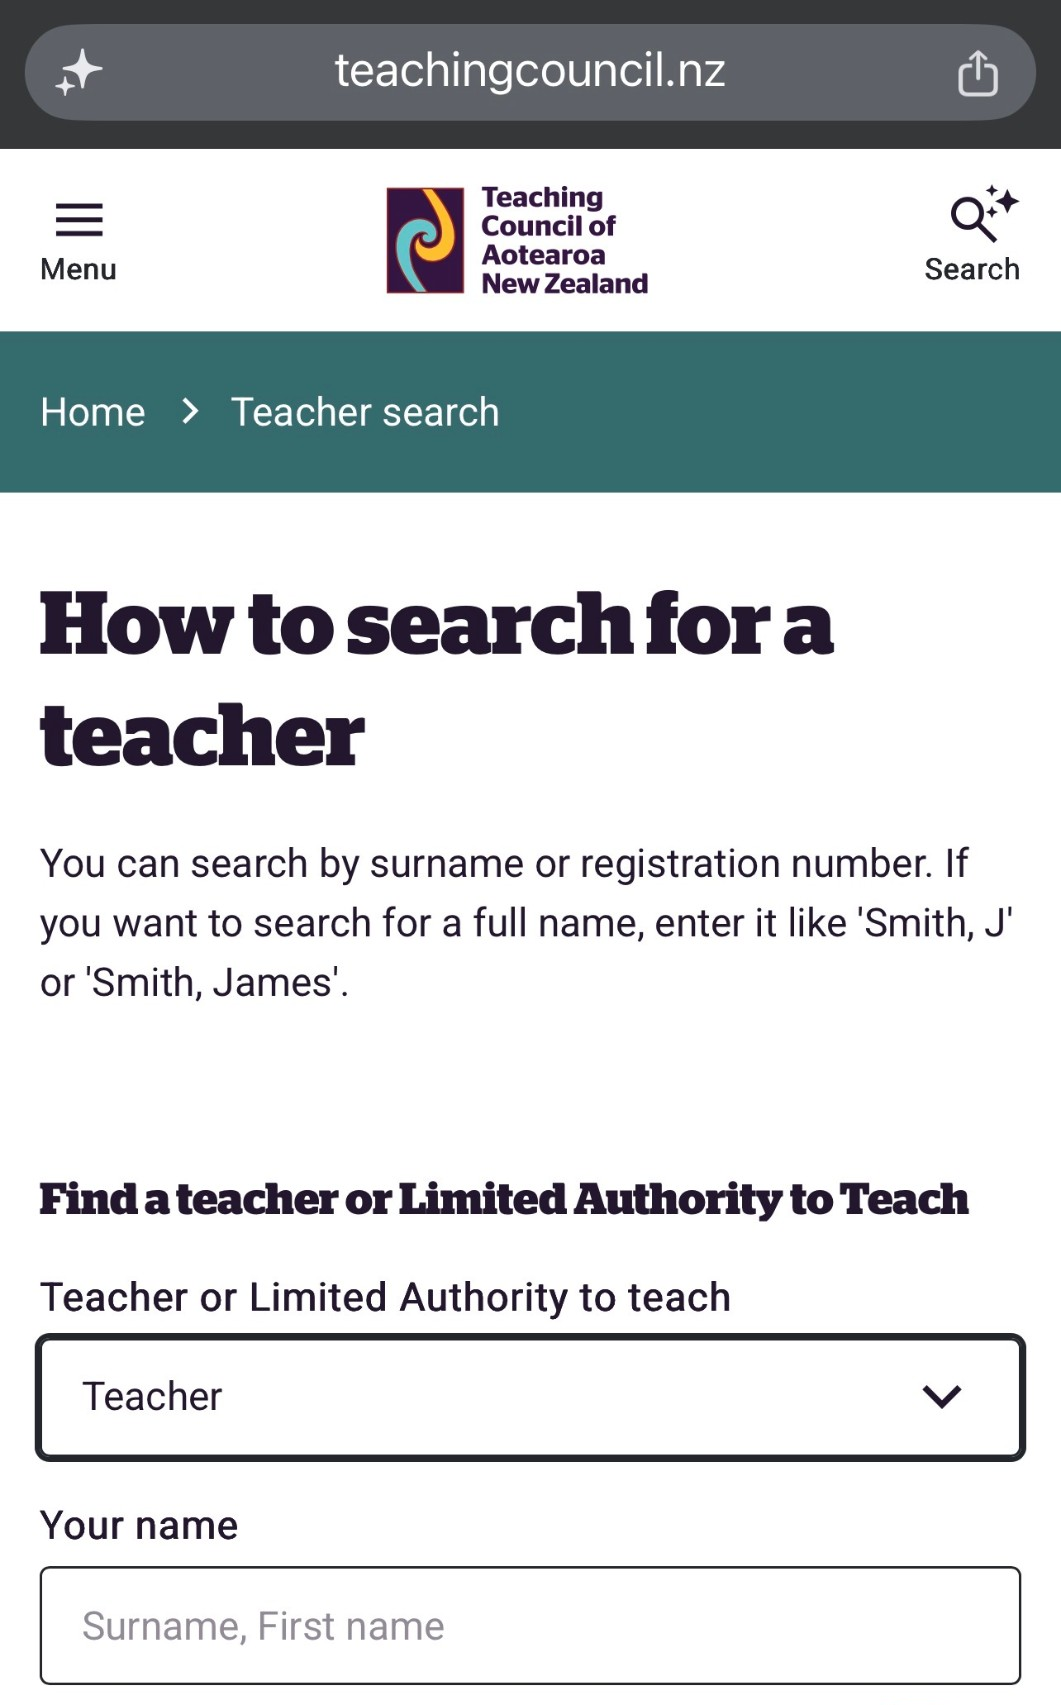
\includegraphics[height=8.6cm]{tutorcheck-tc-02102026}};
\shotframe
\begin{scope}[x={(img.south east)},y={(img.north west)}]
\rbox{0.012}{0.405}{0.975}{0.515}{1}
\rbox{0.025}{0.14}{0.975}{0.22}{2}
\rbox{0.025}{0.004}{0.975}{0.092}{3}
\end{scope}\end{tikzpicture}\par
\srcnote{截图：Teaching Council 官网 Teacher search 页}
\medskip\raggedright
{\large\rnum{1}\ 格式：姓, 名（如 \textbf{Smith, James}）\par}
\smallskip
{\large\rnum{2}\ 下拉框保持 \textbf{Teacher}\par}
\smallskip
{\large\rnum{3}\ 输入名字，点搜索\par}
\medskip
\begin{lcard}[GOLD]\large\centering 重名太多？请老师告诉你\textbf{注册号}，\\同一页输入，结果唯一。\end{lcard}
\end{frame}

% ---------- P6 ② IQA 是什么 ----------
\begin{frame}[plain]
\titlebar{\wnum{2}\ 海外学历 · 在新西兰算几级}
\medskip\centering
\begin{tikzpicture}
\node[anchor=south west,inner sep=0](img) at (0,0){
\includegraphics[height=8.4cm]{tutorcheck-nzqa1-02102026}};
\shotframe
\begin{scope}[x={(img.south east)},y={(img.north west)}]
\rbox{0.28}{0.925}{0.72}{0.975}{1}
\rbox{0.05}{0.375}{0.95}{0.585}{2}
\end{scope}\end{tikzpicture}\par
\srcnote{截图：NZQA（新西兰学历评估局）官网}
\medskip\raggedright
{\large\rnum{1}\ 网址认准 \textbf{nzqa.govt.nz}\par}
\smallskip
{\large\rnum{2}\ \textbf{IQA}：海外学位对照新西兰 1–10 级\par}
\medskip
\begin{lcard}\centering
{\large\bfseries\textcolor{NAVY}{7 级 = 学士 ｜ 9 级 = 硕士}}\\[1mm]
{\large\bfseries\textcolor{ACCENT}{10 级 = 博士（最高一级）}}
\end{lcard}
\end{frame}

% ---------- P7 ② 要原始 PDF ----------
\begin{frame}[plain]
\titlebar{\wnum{2}\ 要原始 PDF，不要截图}
\medskip\centering
\begin{tikzpicture}
\node[anchor=south west,inner sep=0](img) at (0,0){
\includegraphics[height=7.2cm]{tutorcheck-nzqa2-02102026}};
\shotframe
\begin{scope}[x={(img.south east)},y={(img.north west)}]
\rbox{0.06}{0.275}{0.93}{0.56}{1}
\rbox{0.10}{0.015}{0.90}{0.085}{2}
\end{scope}\end{tikzpicture}\par
\srcnote{截图：NZQA 官网 Check a document online 页}
\medskip\raggedright
\begin{lcard}
{\large\rnum{1}\ \textbf{网站只认这样的文件：}}\\[1mm]
\hspace*{7mm}原始 PDF ｜ 没改过一处\\
\hspace*{7mm}从 NZQA 网站直接下载 ｜ 文件名没动过
\end{lcard}
{\large\rnum{2}\ 上传文件，网站\textbf{自动核对}\par}
\medskip
\begin{goldbox}\centering{\large\bfseries\textcolor{NAVY}{请老师发文件本身}}\\[1mm]{\large\bfseries\textcolor{ACCENT}{截图、照片、打印件都验不了}}\end{goldbox}
\end{frame}

% ---------- P8 我的判断 ----------
\begin{frame}[plain]
\stepchip{我的判断}
\medskip
\titlebar{查得到，只是底线}
\bigskip
\begin{lcard}
{\large\bfseries 查不到 $\neq$ 不能请}\\[1mm]
{\large 不少大学生家教没有教师注册，\\[0.5mm]也教得很好。}
\end{lcard}
\medskip
\begin{lcard}
{\large\bfseries 但说了，就该对得上}\\[1mm]
{\large 简介写「在职老师」→ 名字查得到\\[0.5mm]简介写「海外博士」→ 拿得出 PDF}
\end{lcard}
\medskip
\begin{lcard}
{\large\bfseries 开口问，不失礼}\\[1mm]
{\large 有资质的老师，通常不介意你核对，\\[0.5mm]反而会觉得你是认真选老师的家长。}
\end{lcard}
\bigskip
\begin{goldbox}\centering{\Large\bfseries\textcolor{NAVY}{核对的不是「有没有」}}\\[1.5mm]{\Large\bfseries\textcolor{ACCENT}{是「说的和查到的」}}\\[1mm]{\Large\bfseries\textcolor{ACCENT}{对不对得上}}\end{goldbox}
\end{frame}

% ---------- P9 Takeaway ----------
{\setbeamercolor{background canvas}{bg=NAVY}
\begin{frame}[plain]\color{white}\centering
\vfill{\LARGE\bfseries 资质不是写出来的，}\\[2mm]{\LARGE\bfseries 是查出来的}
\vfill
{\Large 教师注册：一个名字就能查}\\[3mm]
{\Large 海外学历：要原始 PDF}\\[3mm]
{\Large 对得上，比写得多更重要}
\vfill{\large\color{SOFTBG} 新西兰高中补习 · 家长核验指南}
\vfill\vfill\end{frame}}

% ---------- P10 家长反思句 ----------
\begin{frame}[plain]\centering
\vfill
{\fontsize{26}{36}\selectfont\bfseries\textcolor{NAVY}{孩子的补习老师，}\\\textcolor{ACCENT}{你查过名字吗？}\par}
\vfill
\begin{softcard}\large 我的教师注册和学历认证，\\都可以线下当面核验。\end{softcard}
\vfill\vfill
\end{frame}

\end{document}
